\section{Results}
\label{sec:dihiggs_result}
%-------------------------------------------------------------------------------

The data yields observed in all
signal regions are in good agreement with the background
expectations. In order to quantify the compatibility of the observed
dataset with a signal of a given cross section $\sigma_{H}$ limits on
$pp \to hh$  production were set as a function of  $m_{hh}$ in the
range 500 GeV to 3000 GeV.

A simultaneous maximum-likelihood fit for the number of events
in the signal region and one of the top control regions is performed. The fit
includes six contributions: signal, $W$+jets, $Z$+jets, $t\bar{t}$ ,
single-top, di-boson and multi-jet. The $t\bar{t}$ normalisation is free to float in
the global fit while the di-boson, $W$+jets, $Z$+jets and multi-jet
backgrounds are constrained to the expected Standard Model cross
section within their uncertainties.

The fit is performed combining  electron and muon
channels in one single data yield. Systematic uncertainties are taken into account as nuisance
parameters with Gaussian sampling distributions. For each source of
systematic uncertainty, the correlations across bins and between
different kinematic regions, as well as those between signal and
background, are taken into account. 

Limits on resonant $hh\rightarrow bbWW$ production are set by performing
counting experiments over relevant ranges of $m_{hh}$\footnote{Each $m_{hh}$
range has been determined keeping the efficiency at 75\% as was agreed upon
during unblinding approval with 2015 data}. Limits are set on resonant
production over a range of $m_X$ = [500, 3000] GeV{\footnote{The non-resonant analysis suffered from very low MC statistics, and hence we have agreed to drop it for the CONF note and return to it for the paper.}}.

The statistical analysis of the final results are based on the WSMaker
framework used in previous Run1 Higgs~~\cite{Aad:2012an} and
dihiggs~~\cite{Aad:2052848} analyses. Fitting and input models are handled
by the RooStats~~\cite{2010acat.confE..57M} and
RooFit~~\cite{2003physics...6116V} packages. Complete information about
the statistical treatment and asymptotic formulae used to calculate the
limits can be found in ~~\cite{Cowan:2010js}. Profile-likelihood-ratio test
statistics are used to measure the compatibility of the background-only
hypothesis with the observed data and to test the hypothesis of Higgs
boson pair production with its cross section as the parameter of interest.
The likelihood is the product of terms of the Poisson probability
constructed from the final discriminant and of nuisance parameter
constraints with either Gaussian, log-normal, or Poisson distributions.
Upper limits on the Higgs boson pair production cross section are derived
using the CL$_\text{s}$ method~~\cite{0954-3899-28-10-313}.

The expected upper limit at 95\% CL on the cross-section of
resonant production as a function of mass is shown in
Figure ~\ref{fig:finalLimit}. 
The most stringent limit is observed (expected) for a resonant mass of
$\sim$900 (900) GeV at $\sim$0.9 (0.6) pb. In appendix \ref{app:StatFit} we
report pull plots and ranking plots for all systematics included in
the fit as fit healthiness tests.


\begin{figure}[!h]
\begin{center}
%\includegraphics*[width=0.60\textwidth] {chapters/dihiggs/figures/limit_2015plus2016_SRandCRsysts.png}
%\includegraphics*[width=0.60\textwidth] {chapters/dihiggs/figures/limit_sep15_splitLoHiSelections.png}
\includegraphics*[width=0.60\textwidth] {chapters/dihiggs/figures/limit_observed_1300swap.png}
\caption[Expected upper limit at 95\% CL on the cross-section of resonant
production.]{Expected upper limit at 95\% CL on the cross-section of resonant
production.}
\label{fig:finalLimit}
\end{center}
\end{figure}

\begin{figure}[hb]
\begin{center}
  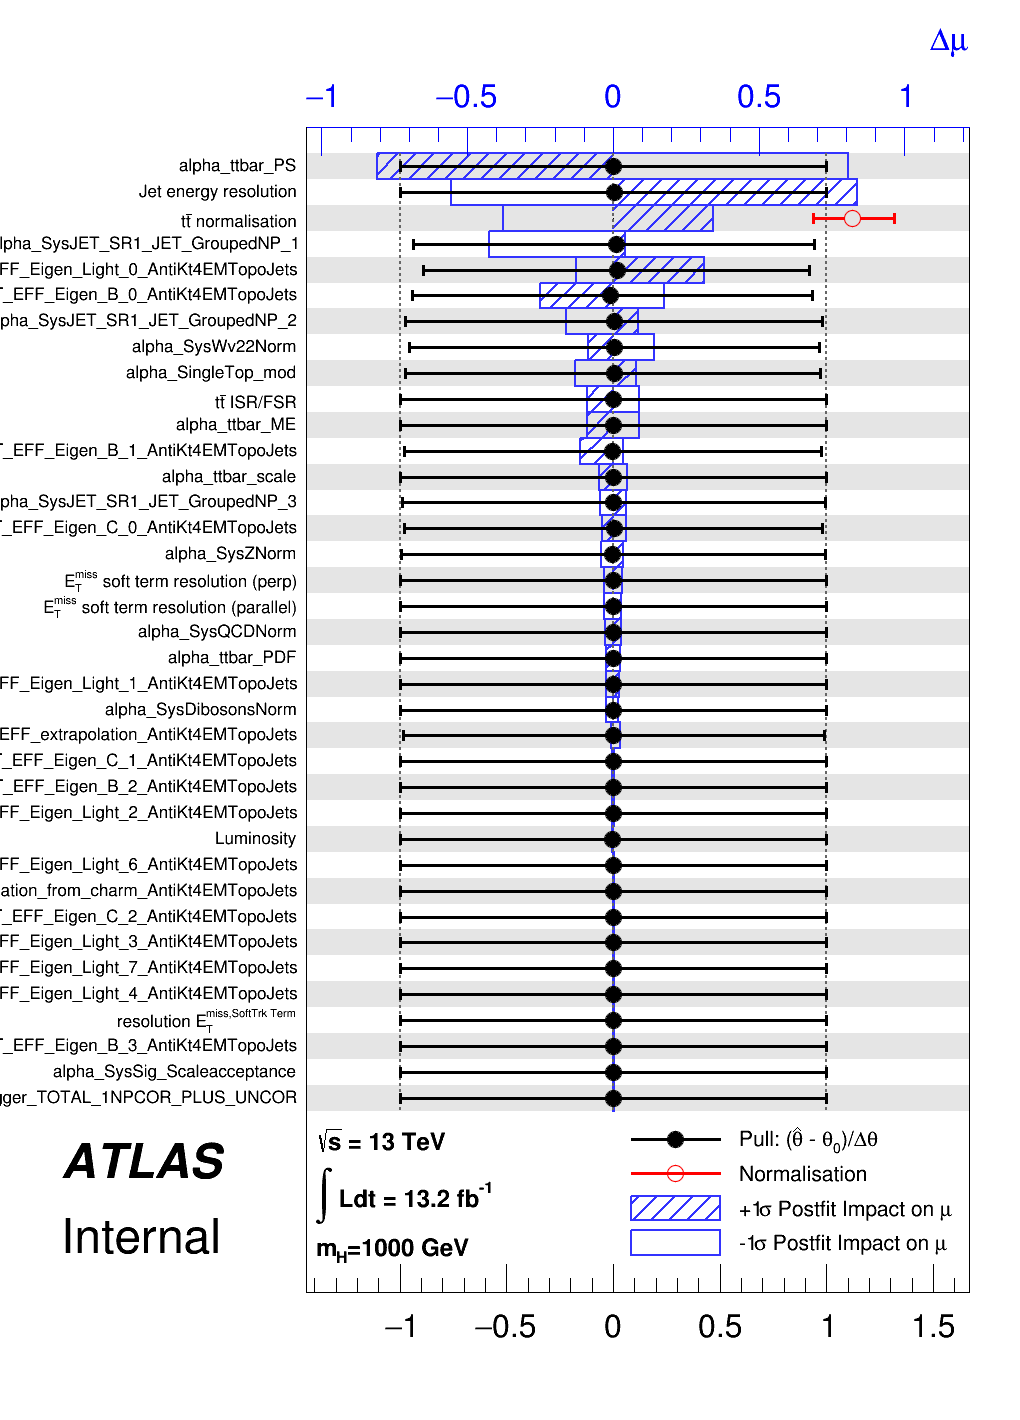
\includegraphics[width=.75\textwidth]{chapters/dihiggs/figures/statFit_appendix/80009_260916-v3-observedPullPlots-x1000_HH_13TeV_260916-v3-observedPullPlots-x1000_Systs_1000_pulls_1000.png}
  \caption{NP ranking plot for m$_X = 1000$ GeV produced when fitting to data in the control region and signal region.}
  \label{fig:npRanking_1000}
\end{center}    
\end{figure}

% Future additions to the analysis that increase signal purity and/or further
% reduce the backgrounds could allow for limits to be set using a shape analysis.
  
\clearpage
